% The Clever Algorithms Project: http://www.CleverAlgorithms.com
% (c) Copyright 2011 Jason Brownlee. Some Rights Reserved. 
% This work is licensed under a Creative Commons Attribution-Noncommercial-Share Alike 2.5 Australia License.

% Name
% The algorithm name defines the canonical name used to refer to the technique, in addition to common aliases, abbreviations, and acronyms. The name is used in terms of the heading and sub-headings of an algorithm description.
\section{Golden Section Search} 
\label{sec:golden_section_search}
\index{Golden Section Search}
\index{Golden Mean Search}

% other names
% What is the canonical name and common aliases for a technique?
% What are the common abbreviations and acronyms for a technique?
\emph{Golden Section Search, Golden Mean Search.}

% Taxonomy: Lineage and locality
\subsection{Taxonomy}
\index{Line Search}
\index{Direct Search}
\index{Pattern Search}
\index{Global Optimization}
% To what fields of study does a technique belong?
Golden Section Search is a Line Search method for Global Optimization in one-dimension. It is a Direct Search (Pattern Search) method as it samples the function to approximate a derivative rather than computing it directly.
% What are the closely related approaches to a technique? 
The Golden Section Search is related to pattern searches of discrete ordered lists such as the Binary Search and the  Fibonacci Search. It is related to other Line Search algorithms such as Brent's Method and more generally to other direct search optimization methods such as Gradient Descent.

% Strategy: Problem solving plan
% The strategy is an abstract description of the computational model. The strategy describes the information processing actions a technique shall take in order to achieve an objective. The strategy provides a logical separation between a computational realization (procedure) and a analogous system (metaphor). A given problem solving strategy may be realized as one of a number specific algorithms or problem solving systems. The strategy description is textual using information processing and algorithmic terminology.
\subsection{Strategy}
% What is the information processing objective of a technique?
The information processing objective of the method is to locate the extremum of a function.
% What is a techniques plan of action?
It does this by directly sampling the function using a pattern of three points. The points form the brackets on the search, the first and the last the current bounds of the search, and the third point that partitions the intervening space. The partitioning point is selected so that the ratio between the larger partition and the whole interval is the same as the ratio of the larger partition to the small partition, known as the golden ratio ($\phi$). The partitions are compared based on their function evaluation and the better performing section is selected as the new bounds on the search. The process recurses until the desired level of precision (bracketing of the optimum) is obtained or the search stalls.

% Heuristics: Usage guidelines
% The heuristics element describe the commonsense, best practice, and demonstrated rules for applying and configuring a parameterized algorithm. The heuristics relate to the technical details of the techniques procedure and data structures for general classes of application (neither specific implementations not specific problem instances). The heuristics are described textually, such as a series of guidelines in a bullet-point structure.
\subsection{Heuristics}
% What are the suggested configurations for a technique?
% What are the guidelines for the application of a technique to a problem instance?

\begin{itemize}
	\item Assumes that the function is convex and unimodal specifically, that the function has a single optimum and that it lies between the first two bracket points.
	\item Intended to find the extrema one-dimensional continuous functions.
	\item It was shown to be more efficient than equal-sized partition line search.
	\item The termination criteria is a specification on the minimum distance between the brackets on the optimum.
	\item It can quickly locate the bracketed area of the optimum but is less efficient at locating the specific optimum.
	\item Once a solution of desired precision is located, it can be provided as the basis to a second search algorithm that has a faster rate of convergence.
\end{itemize}

% sample script in R
\subsection{Code Listing}
% listing
Listing~\ref{stats_golden_section_search} provides a code listing Golden Section Search method in R solving a one-dimensional nonlinear unconstrained optimization function. Figure~\ref{plot:golden_section_search_result} provides a plot of the test problem with the located minimum highlighted.

% algorithm and package
The example uses the {optimize()} function in the \texttt{stats} core package \cite{RDevelopmentCoreTeam2011a}. This function uses a Golden Section Search with successive Parabolic Interpolation. This combination of a linear search followed successively by Parabolic Interpolation is a common pattern for improving the overall result by leveraging the non-parametric nature of the former and the speed of convergence of the latter methods. The \texttt{optimize()} function is for One-Dimensional Optimization, for more information on this library type: \texttt{library(help="stats")}, and for more information on the function type: \texttt{?optimize}.

% problem
The test problem is the basin function in one-dimension where the optimum is at $f(0)=0$ and the domain is defined as $x \in [-5,5]$. 

\lstinputlisting[firstline=7,language=r,caption={Example of Golden Section Search in R using the \texttt{optimize()} function in the \texttt{stats} core package.}, label=stats_golden_section_search]{../src/algorithms/optimization/stats_golden_section_search.R}

\begin{figure}[htp]
\centering
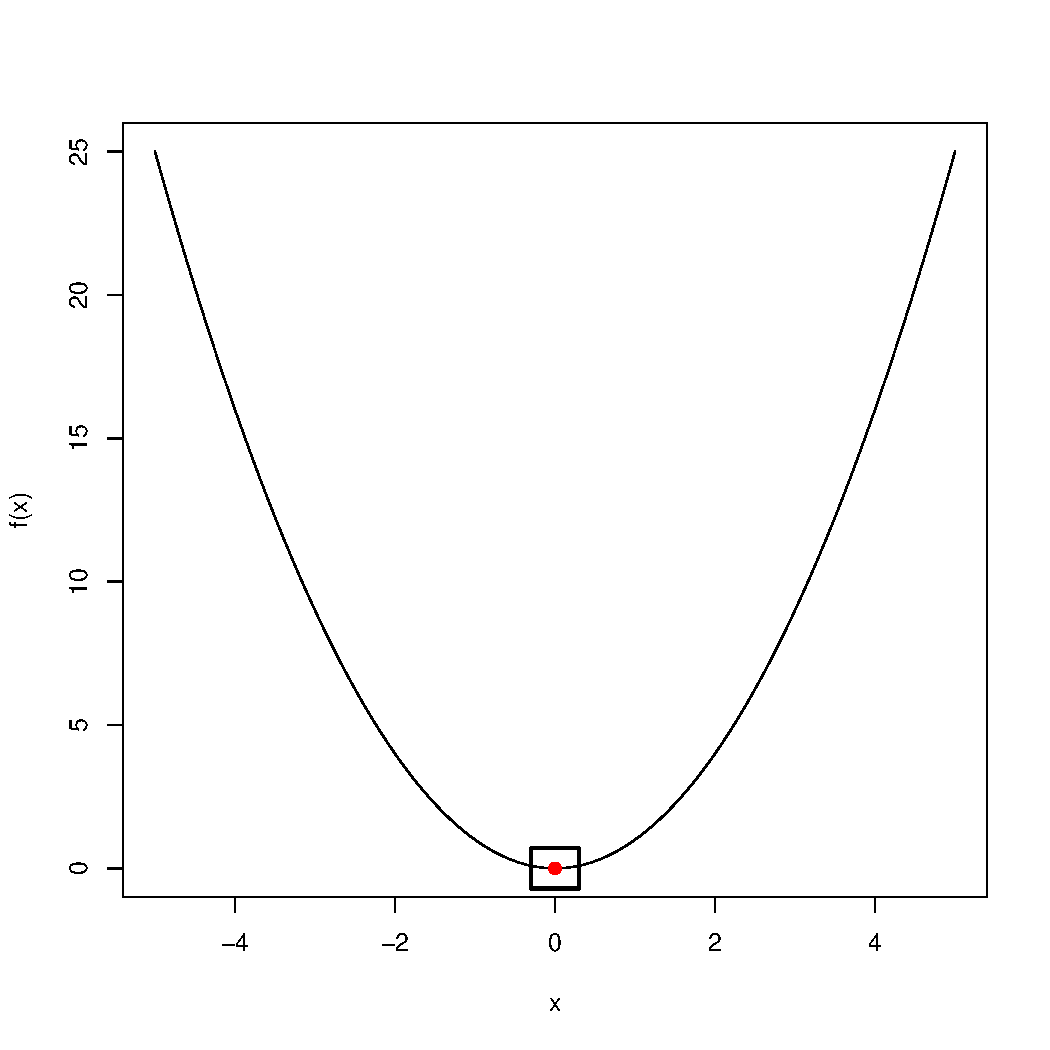
\includegraphics[scale=0.45]{a_optimization/golden_section_search_result.pdf}
\caption{Plot of the basin function in one-dimension with the located minimum highlighted.}
\label{plot:golden_section_search_result}
\end{figure}

The \texttt{stats} core package also provides an implementation of Brent's method in the \texttt{optim} function.

% References: Deeper understanding
% The references element description includes a listing of both primary sources of information about the technique as well as useful introductory sources for novices to gain a deeper understanding of the theory and application of the technique. The description consists of hand-selected reference material including books, peer reviewed conference papers, journal articles, and potentially websites. A bullet-pointed structure is suggested.
\subsection{References}
% What are the primary sources for a technique?
% What are the suggested reference sources for learning more about a technique?

% primary sources
\subsubsection{Primary Sources}
% seminal
The method was described by Kiefer in 1953 as a method for finding the maximum of a function without regularity conditions such as continuity and function derivatives \cite{Kiefer1953}.
Johnson provided an early description of the method in a technical report for RAND Corporation \cite{Johnson1955}.

% more info
\subsubsection{More Information}
% useful
Press et~al.\ provide a terse and practical introduction to the method with well-commented sample code in the C programming language \cite{Press2007}.
% early
Brent provides an early treatment of the method is his text on minimization without derivatives \cite{Brent1973}.
% text books
Many text books on scientific computing or numerical analysis include a section on Golden Section Search, for example, see Heath \cite{Heath2002}.

% END
